\section{Introduction}
%uvod
\begin{frame}
	\frametitle{Autonomous exploration}
	\begin{itemize}
%		\item[-] \textbf{Autonomous exploration} - the ability of robots to autonomously travel around an unknown environment gathering the necessary information to obtain a useful map for navigation\footcite{Julia2012}
		\item[-] \textbf{Multi-robot system} 
		\item[-] \textbf{Coordinated} robots 
		\item[-] \textbf{Goal:} minimize the overall exploration time
	\end{itemize}
	\begin{figure}	
	\centering
	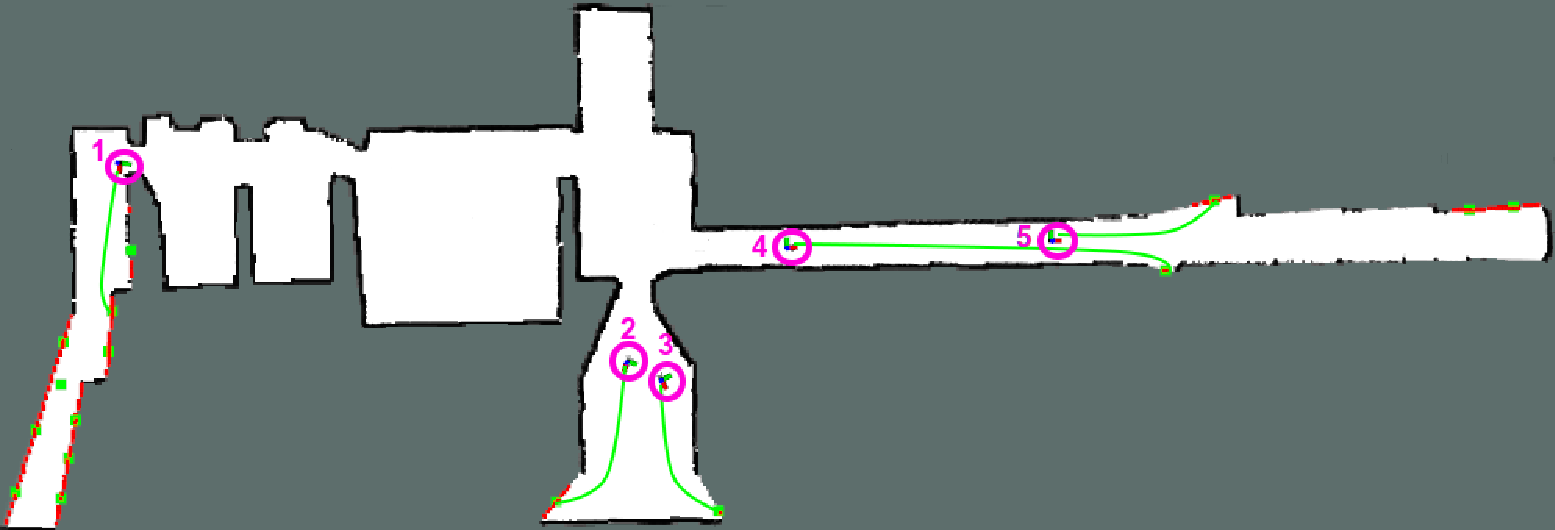
\includegraphics[width=0.85\textwidth]{figures/siminprogress1}
	%\caption{Autonomous exploration using multi-robot system. Mobile robots focused on different target points according to an exploration strategy.}
	\end{figure}
\end{frame}

\begin{frame}
	\frametitle{Multi-robot exploration}
	\begin{itemize}
		\item[-] \textbf{ADVANTAGES:}
		\begin{itemize}
			\item[-] Robustness %(due to redundancy)
			\item[-] Efficiency %(a robot team can accomplish a predefined task much quicker than a single robot can\footcite{Dias2000})
			\item[-] Sensor fusion\footcite{Wurm2008} %(can compensate sensor uncertainty)
%			\item[-] Free from single-point failure (if system is decentralized)
			\item[-] Larger range of task domains\footcite{Dias2006}
		\end{itemize}
		\item[-] \textbf{DISADVANTAGES:}
		\begin{itemize}
			\item[-] High communication requirement% in general
			\item[-] If greedy assignment methods are used, convergence to a suboptimal goal is possible
		\end{itemize} 
	\end{itemize}
\end{frame}

\begin{frame}
	\frametitle{Problem formulation}
%		\item[-] The goal of an exploration strategy consists in increasing robots knowledge of the environment by selecting appropriate control actions with the objective to minimize the size of the unexplored area. 		
	\begin{columns}
		\begin{column}{0.5\textwidth}
			\begin{itemize}
				\item[-] Given a team of $n$ robots ($r_{1}$,...,$r_{n}$), the goal of the exploration	strategy is twofold:
				\begin{itemize}
					\item[1)] \textbf{Compute effective targets} ($w_{1}$,...,$w_{m}$) 
					\item[2)] \textbf{Coordination strategy:} which robot to which target 
				\end{itemize}			
			\end{itemize}
		\end{column}
		\begin{column}{0.5\textwidth}  %%<--- here
			\begin{center}
				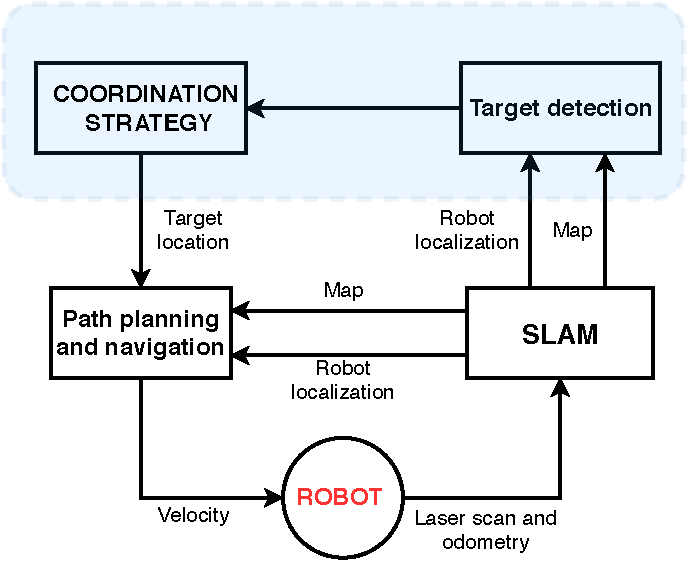
\includegraphics[width=1\textwidth]{figures/strategy_all}
				\label{fig:gauss}
			\end{center}
		\end{column}
	\end{columns}	
\end{frame}

%\begin{frame}
%	\frametitle{Problem formulation (2)}
%	\begin{figure}
%		\centering
%		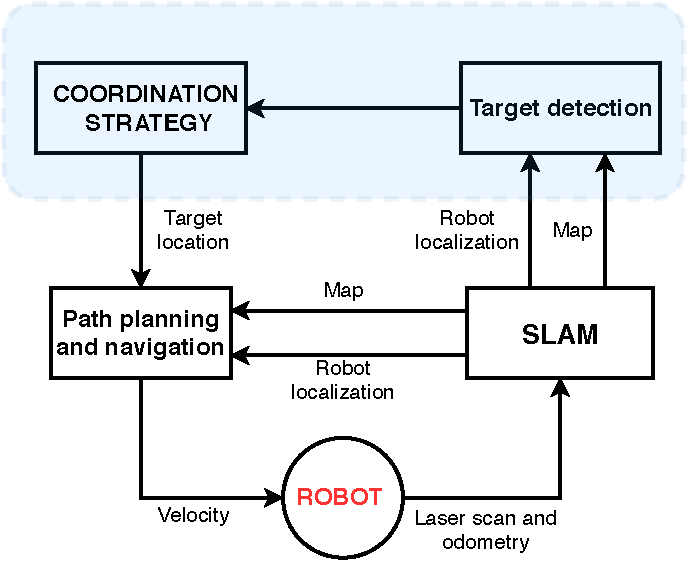
\includegraphics[width=0.6\textwidth]{figures/strategy_all}
%		\caption{The overall frontier exploration and mapping process for a single robot that can be easy extended to multi-robot system.}
%	\end{figure}
%\end{frame}

\begin{frame}
	\frametitle{Computing effective targets - frontier detection (1)}
	\begin{itemize}
		\item[-] \textbf{Occupancy grid map} - discretizes the environment into a grid of map cells\footcite{Moravec}
		\item[-] \textbf{Free, occupied or unknown}
		\item[-] \textbf{Frontier} introduced by Yamauchi\footcite{Yamauchi1997} 				
	\end{itemize}
	\begin{figure}
		\centering
		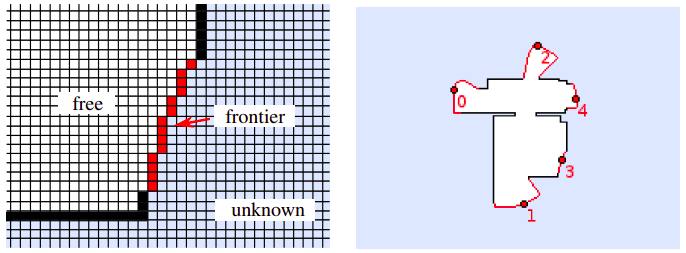
\includegraphics[width=0.75\textwidth]{figures/environment1}
		%\caption{2D occupancy grid map: unknown cells are shown light blue, free cells are depicted in white and occupied cells (obstacles) in black. Left: Frontier cells (red) are determined at the boundary between free and unknown map cells. Right: Five exploration targets, visualized as red circles, are generated at frontiers (Source\footcite{Wurm2012})}
	\end{figure}
\end{frame}

\begin{frame}
	\frametitle{Computing effective targets - frontier detection (2)\footcite{Umari2017}$\,$\footcite{Orsulic2019}}
		\begin{columns}
				\begin{column}{0.5\textwidth}\centering
					{\bf{RRT frontier detection}}\\ 
					\vspace{0.2cm}
					\begin{center}
						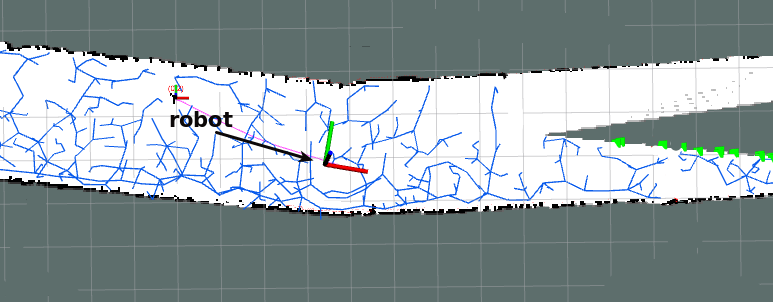
\includegraphics[height=2.3cm]{figures/rrt2}
						%\caption{Industrial Manipulator KUKA KR30}
						\label{fig:cent}
					\end{center}
					\vspace{0.1cm}
					%\begin{itemize}
						%\item[-] RRT frontier detection%\footcite{Umari2017}
					%\end{itemize}
				\end{column}
				\begin{column}{0.5\textwidth}\centering
					{\bf{Efficient dense frontier detection}}\\ 
					\vspace{0.2cm}
					\begin{center}
						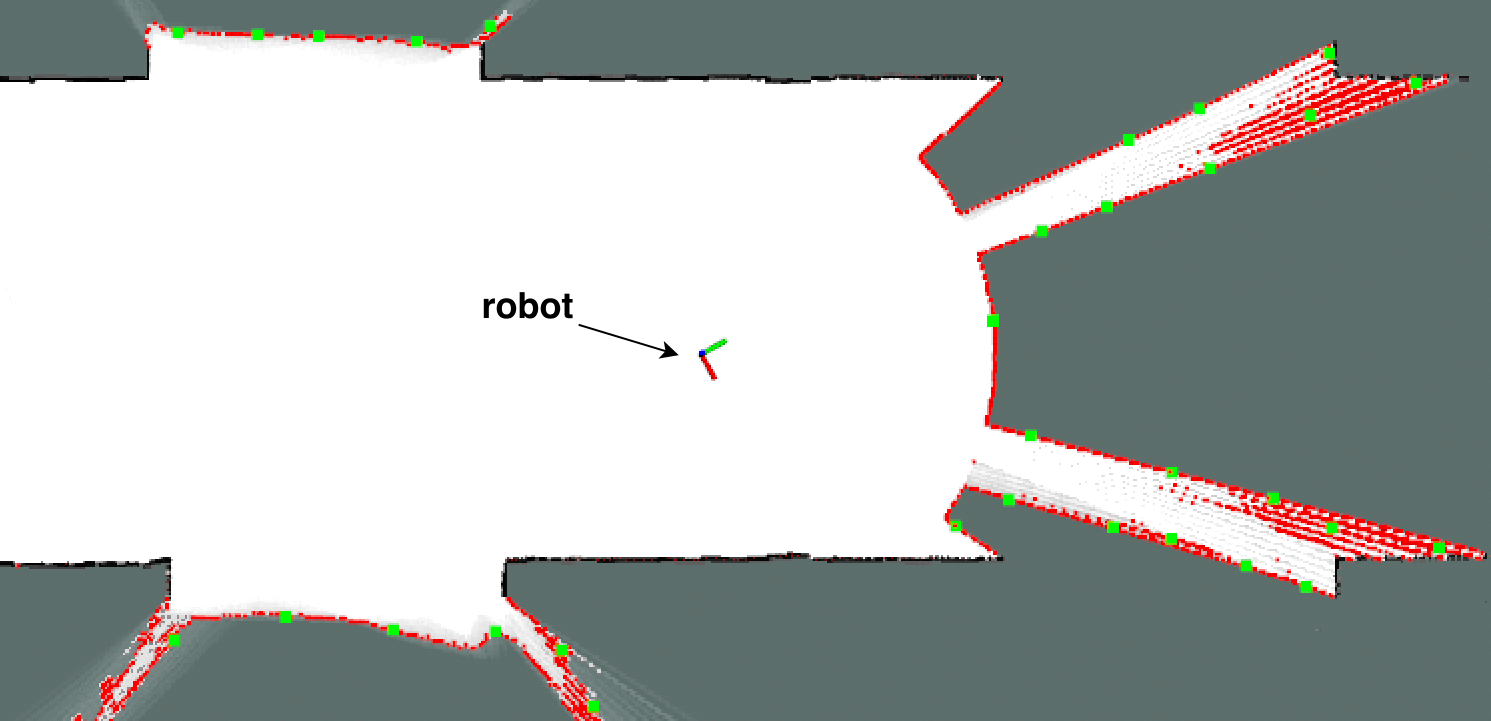
\includegraphics[height=2.3cm]{figures/carto1}
						%  \caption{Collaborative Manipulator KUKA IIWA}
						\label{fig:decent}
					\end{center}
				\end{column}
			\end{columns}
\end{frame}
		
\begin{frame}
	\frametitle{Coordination algorithms}
		\begin{figure}
			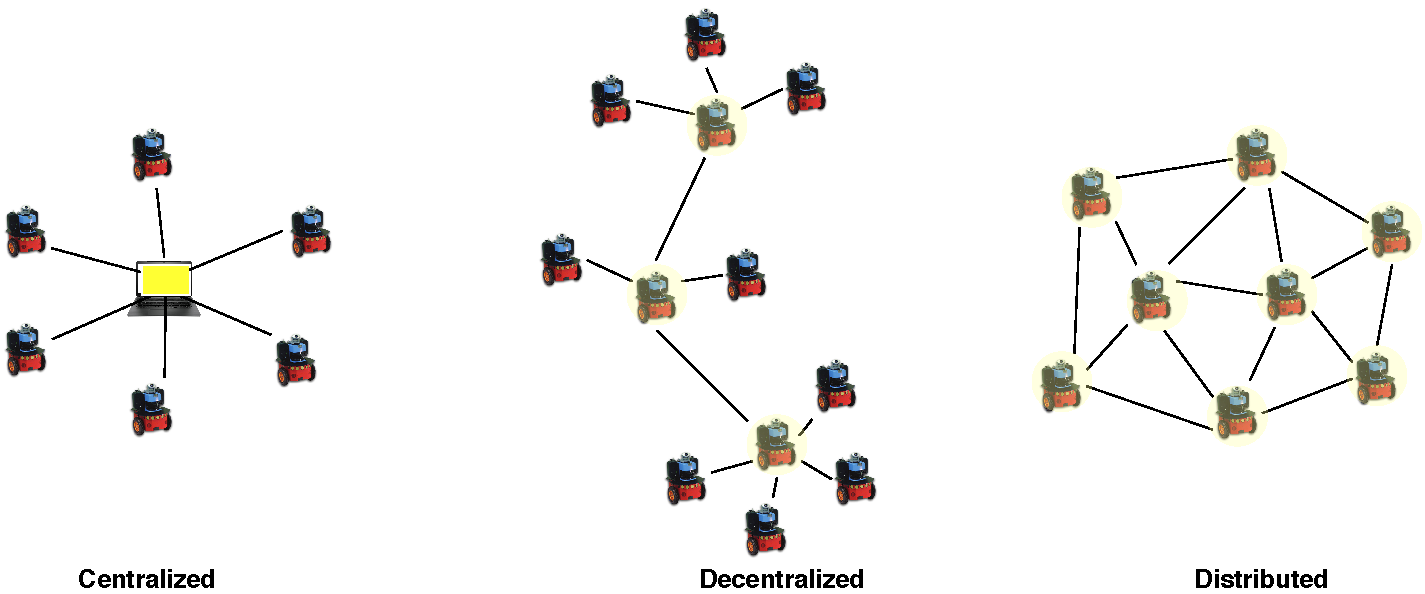
\includegraphics[width=1\textwidth]{figures/robots}
			%\caption{Industrial Manipulator KUKA KR30}
			\label{fig:cent}
		\end{figure}
%	\begin{columns}
%		\begin{column}{0.5\textwidth}\centering
%			{\bf{Centralized}}\\ 
%			\vspace{0.1cm}
%			\begin{center}
%				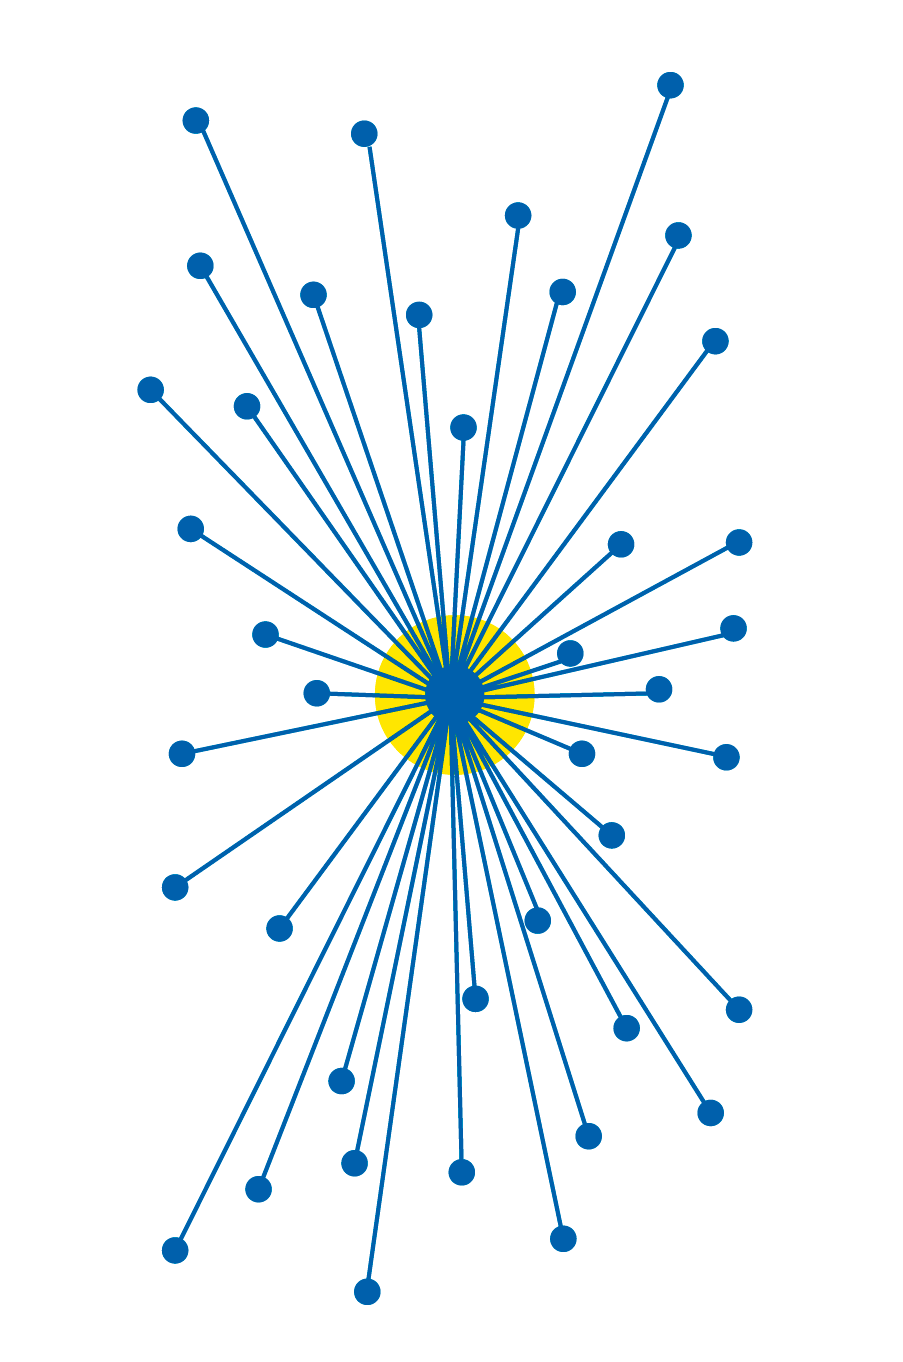
\includegraphics[height=3cm]{figures/cent}
%				%\caption{Industrial Manipulator KUKA KR30}
%				\label{fig:cent}
%			\end{center}
%			\vspace{0.01cm}
%			\begin{itemize}
%				\item[-] Single central \textit{leader}
%				\item[-] Communication limits and robustness issues 
%				\item[-] Optimal plans can be found
%			\end{itemize}
%		\end{column}
%		\begin{column}{0.5\textwidth}\centering{\bf{Decentralized }}\\
%			\vspace{0.1cm}
%			\begin{center}
%				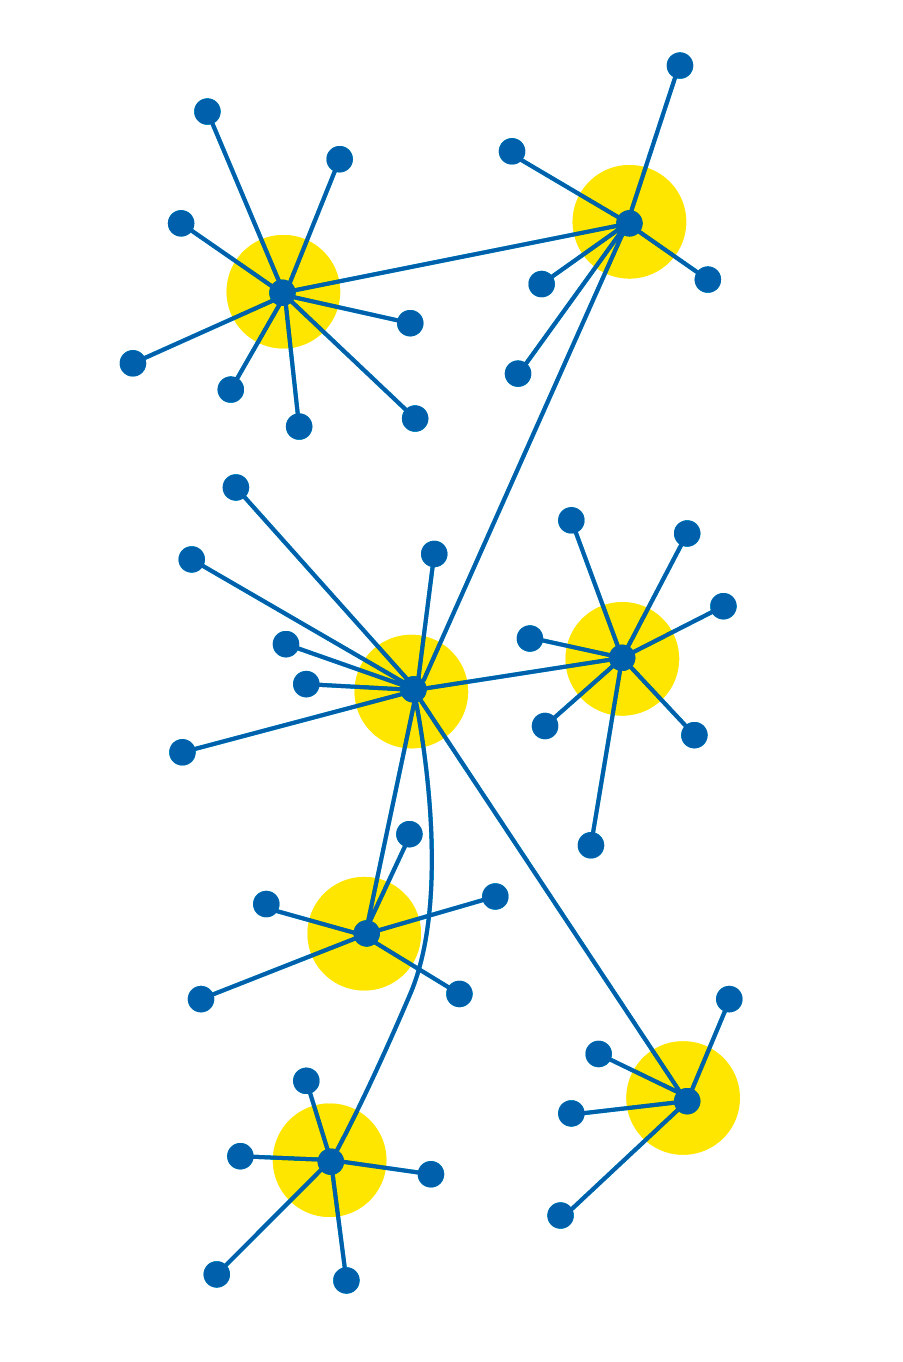
\includegraphics[height=3cm]{figures/decent}
%				%  \caption{Collaborative Manipulator KUKA IIWA}
%				\label{fig:decent}
%			\end{center}
%			\vspace{0.01cm}
%			\begin{itemize}
%				\item[-] Robots are completely (or at least partially) independent
%				\item[-] Better reliability, flexibility, adaptability and robustness
%			\end{itemize}
%		\end{column}
%	\end{columns}
	
\end{frame}


%\begin{frame}
%	\frametitle{Motivation}
%	\begin{columns}
%		\begin{column}{0.5\textwidth}
%			\begin{itemize}
%				\item Industrial scenario : Delicate sanding of complex shape surfaces in aerial industry 
%				\item Robot sanding using Kuka KR30 equipped with ACF (Active Contact Flange)
%				\item Goal: Create robotic sanding system capable to control contact force in 6 DOF
%			\end{itemize}
%		\end{column}
%		\begin{column}{0.5\textwidth}  %%<--- here
%			\begin{center}
%				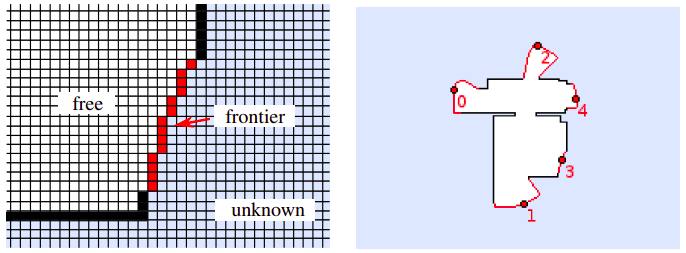
\includegraphics[width=1\textwidth]{figures/environment1}
%				\label{fig:enikon_kuka}
%			\end{center}
%		\end{column}
%	\end{columns}
%\end{frame}
%\begin{frame}
%     \frametitle{Effective Robotic GriNDing of Surface Areas through HORSE framework (ENDORSE)}
%     \begin{columns}
%        \begin{column}{0.3\textwidth}
%            \begin{itemize}
%                 \item \textbf{Compliant control algorithm}
%                 \item Human oriented machine interface
%                 \item Safety of human
%                 \item Automated quality inspection system
%            \end{itemize}
%        \end{column}
%        \begin{column}{0.7\textwidth}  %%<--- here
%            \begin{center}
%             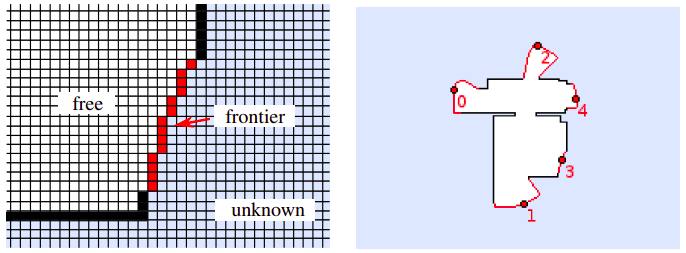
\includegraphics[width=1\textwidth]{figures/environment1}
%            %  \caption{ENDORSE setup}
%             \label{fig:enikon_kuka}
%             \end{center}
%        \end{column}
%    \end{columns}
%\end{frame}
